\documentclass[12pt,a4paper]{article}
\usepackage[utf8]{utf8}
\usepackage[margin=1in]{geometry}
\usepackage{tcolorbox}
\usepackage{tikz}
\usetikzlibrary{shapes.geometric, arrows.meta, positioning}

\title{\textbf{The Ailing Planet: the Green Movement's Role}\\[0.3em] \Large Textbook Page 37}
\author{\textbf{Author:} Nani Palkhivala \quad|\quad \textbf{Textbook:} Hornbill (Class 11)}
\date{}

\begin{document}

\maketitle

\section*{Text Content}

The following article was written by Nani Palkhivala and published in \textit{The Indian Express} on 24 November 1994. The issues that he raised regarding the declining health of the earth continue to have relevance.

ONE cannot recall any movement in world history which has gripped the imagination of the entire human race so completely and so rapidly as the Green Movement which started nearly twenty-five years ago. In 1972 the world's first nationwide Green party was founded in New Zealand. Since then, the movement has not looked back.

We have shifted one hopes, irrevocably from the mechanistic view to a holistic and ecological view of the world. It is a shift in human perceptions as revolutionary as that introduced by Copernicus who taught mankind in the sixteenth century that the earth and the other planets revolved round the sun. For the first time in human history, there is a growing worldwide consciousness that the earth itself is a living organism — an enormous being of which we are parts. It has its own metabolic needs and vital processes which need to be respected and preserved.

The earth's vital signs reveal a patient in declining health. We have begun to realise our ethical obligations to be good stewards of the planet and responsible trustees of the legacy to future generations.

The concept of sustainable development was popularised in 1987 by the World Commission on Environment and Development. In its report it defined the idea as "Development that meets the needs of the present, without compromising the ability of future generations to meet their needs", i.e., without stripping the natural world of resources future generations would need.

In the zoo at Lusaka, Zambia, there is a cage where the notice reads, 'The world's most dangerous animal'. Inside the cage there is no animal but a mirror where you see yourself. Thanks to the efforts of a number of agencies in different countries, a new awareness has now dawned upon the most dangerous animal in the world. He has realised the wisdom of shifting from a system based on domination to one based on partnership.

\vspace{1cm}

\begin{figure}[htbp]
\centering
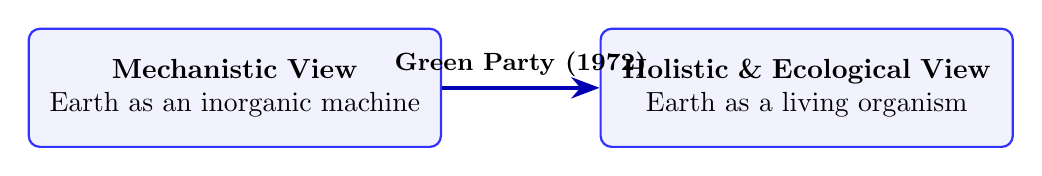
\begin{tikzpicture}[
    box/.style={rectangle, draw=blue!80, fill=blue!5, thick, rounded corners, text width=5cm, align=center, minimum height=1.5cm},
    arrow/.style={-Stealth, ultra thick, draw=blue!70!black}
]
    \node[box] (a) {\textbf{Mechanistic View}\\ Earth as an inorganic machine};
    \node[box, right=2cm of a] (b) {\textbf{Holistic \& Ecological View}\\ Earth as a living organism};

    \draw[arrow] (a) -- node[above, font=\small\bfseries] {Green Party (1972)} (b);
\end{tikzpicture}
\caption{Page 37: The Paradigm Shift in Environmental Perception}
\end{figure}

\end{document}
\documentclass[12pt,a4paper]{article}
\usepackage[utf8]{utf8}
\usepackage[margin=1in]{geometry}
\usepackage{tcolorbox}
\usepackage{tikz}
\usetikzlibrary{shapes.geometric, arrows.meta, positioning}

\title{\textbf{The Ailing Planet: the Green Movement's Role}\\[0.3em] \Large Textbook Page 38}
\author{\textbf{Author:} Nani Palkhivala \quad|\quad \textbf{Textbook:} Hornbill (Class 11)}
\date{}

\begin{document}

\maketitle

\section*{Text Content}

Scientists have catalogued about 1.4 million living species with which mankind shares the earth. Estimates vary widely as regards the still-uncatalogued living species — biologists reckon that about three to a hundred million other living species still languish unnamed in ignominious darkness.

One of the early international commissions which dealt, inter alia, with the question of ecology and environment was the Brandt Commission which had a distinguished Indian as one of its members Mr L.K. Jha. The First Brandt Report raised the question — "Are we to leave our successors a scorched planet of advancing deserts, impoverished landscapes and ailing environment?"

Mr Lester R. Brown in his thoughtful book, \textit{The Global Economic Prospect}, points out that the earth's principal biological systems are four — fisheries, forests, grasslands, and croplands and they form the foundation of the global economic system. In addition to supplying our food, these four systems provide virtually all the raw materials for industry except minerals and petroleum-derived synthetics. In large areas of the world, human claims on these systems are reaching an unsustainable level, a point where their productivity is being impaired. When this happens, fisheries collapse, forests disappear, grasslands are converted into barren wastelands, and croplands deteriorate. In a protein-conscious and protein-hungry world, over-fishing is common every day. In poor countries, local forests are being decimated in order to procure firewood for cooking. In some places, firewood has become so expensive that "what goes under the pot now costs more than what goes inside it". Since the tropical forest is, in the words of Dr Myers, "the powerhouse of evolution", several species of life face extinction as a result of its destruction.

\vspace{1cm}

\begin{figure}[htbp]
\centering
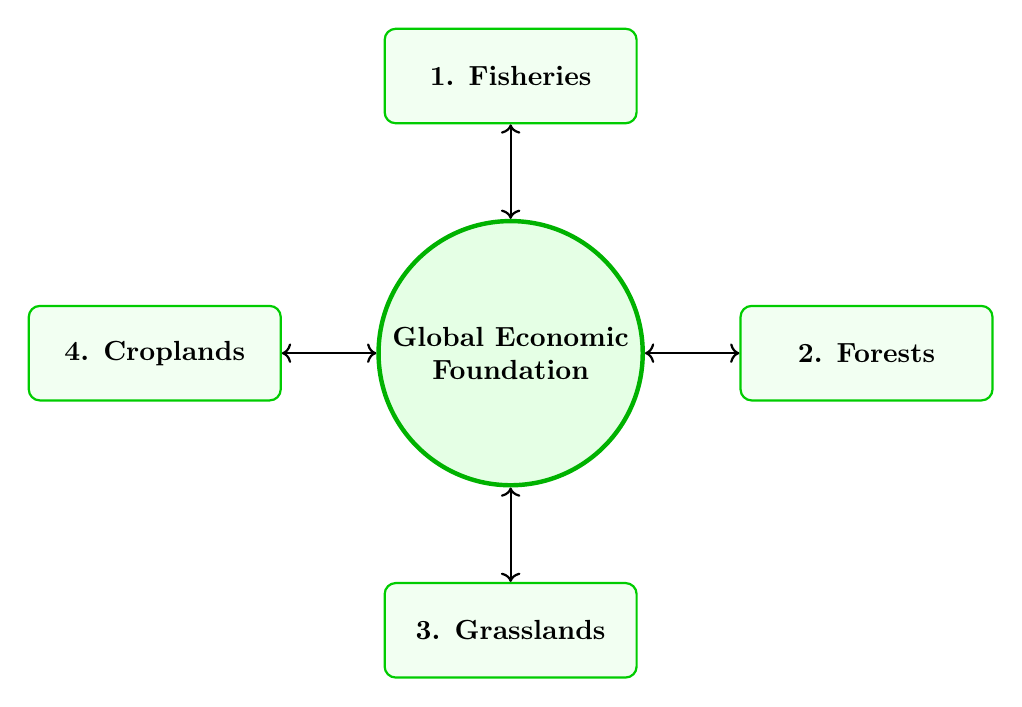
\begin{tikzpicture}[
    center/.style={circle, draw=green!70!black, fill=green!10, ultra thick, minimum size=2.8cm, align=center},
    sys/.style={rectangle, draw=green!80!black, fill=green!5, thick, rounded corners, minimum width=3.2cm, minimum height=1.2cm, align=center}
]
    \node[center] (earth) {\textbf{Global Economic}\\\textbf{Foundation}};
    \node[sys, above=1.2cm of earth] (fish) {\textbf{1. Fisheries}};
    \node[sys, right=1.2cm of earth] (forest) {\textbf{2. Forests}};
    \node[sys, below=1.2cm of earth] (grass) {\textbf{3. Grasslands}};
    \node[sys, left=1.2cm of earth] (crop) {\textbf{4. Croplands}};

    \draw[<->, thick] (earth) -- (fish);
    \draw[<->, thick] (earth) -- (forest);
    \draw[<->, thick] (earth) -- (grass);
    \draw[<->, thick] (earth) -- (crop);
\end{tikzpicture}
\caption{Page 38: Lester R. Brown's Four Biological Systems}
\end{figure}

\end{document}
\documentclass[12pt,a4paper]{article}
\usepackage[utf8]{utf8}
\usepackage[margin=1in]{geometry}
\usepackage{tcolorbox}
\usepackage{tikz}
\usetikzlibrary{shapes.geometric, arrows.meta, positioning}

\title{\textbf{The Ailing Planet: the Green Movement's Role}\\[0.3em] \Large Textbook Page 39}
\author{\textbf{Author:} Nani Palkhivala \quad|\quad \textbf{Textbook:} Hornbill (Class 11)}
\date{}

\begin{document}

\maketitle

\section*{Text Content}

It has been well said that forests precede mankind; deserts follow. The world's ancient patrimony of tropical forests is now eroding at the rate of forty to fifty million acres a year, and the growing use of dung for burning deprives the soil of an important natural fertiliser. The World Bank estimates that a five-fold increase in the rate of forest planting is needed to cope with the expected fuelwood demand in the year 2000.

James Speth, the President of the World Resources Institute, said the other day, "We were saying that we are losing the forests at an acre a second, but it is much closer to an acre-and-a-half to a second".

Article 48A of the Constitution of India provides that "the State shall endeavour to protect and improve the environment and to safeguard the forests and wildlife of the country". But what causes endless anguish is the fact that laws are never respected nor enforced in India. (For instance, the Constitution says that casteism, untouchability and bonded labour shall be abolished, but they flourish shamelessly even after forty-four years of the operation of the Constitution.) A recent report of our Parliament's Estimates Committee has highlighted the near catastrophic depletion of India's forests over the last four decades. India, according to reliable data, is losing its forests at the rate of 3.7 million acres a year. Large areas, officially designated as forest land, "are already virtually treeless". The actual loss of forests is estimated to be about eight times the rate indicated by government statistics.

A three-year study using satellites and aerial photography conducted by the United Nations, warns that the environment has deteriorated so badly that it is 'critical' in many of the eighty-eight countries investigated.

There can be no doubt that the growth of world population is one of the strongest factors distorting the future of human society. It took mankind more than a million years to reach the first billion. That was the world population around the year 1800. By the year 1900, a second billion was added, and the twentieth century has added another 3.7 billion. The present world population is estimated at 5.7 billion. Every four days the world population increases by one million.

\vspace{1cm}

\begin{figure}[htbp]
\centering
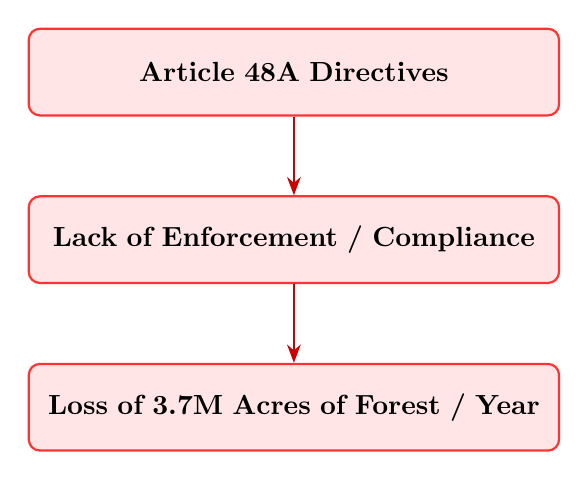
\begin{tikzpicture}[
    node distance=1cm,
    block/.style={rectangle, draw=red!80, fill=red!10, thick, rounded corners, text width=6.5cm, align=center, minimum height=1.1cm},
    arrow/.style={-Stealth, thick, draw=red!80!black}
]
    \node[block] (law) {\textbf{Article 48A Directives}};
    \node[block, below=of law] (gap) {\textbf{Lack of Enforcement / Compliance}};
    \node[block, below=of gap] (loss) {\textbf{Loss of 3.7M Acres of Forest / Year}};

    \draw[arrow] (law) -- (gap);
    \draw[arrow] (gap) -- (loss);
\end{tikzpicture}
\caption{Page 39: Constitutional Directives vs. Actual Deforestation Rate}
\end{figure}

\end{document}
\documentclass[12pt,a4paper]{article}
\usepackage[utf8]{utf8}
\usepackage[margin=1in]{geometry}
\usepackage{tcolorbox}
\usepackage{tikz}
\usetikzlibrary{shapes.geometric, arrows.meta, positioning}

\title{\textbf{The Ailing Planet: the Green Movement's Role}\\[0.3em] \Large Textbook Page 40}
\author{\textbf{Author:} Nani Palkhivala \quad|\quad \textbf{Textbook:} Hornbill (Class 11)}
\date{}

\begin{document}

\maketitle

\section*{Text Content}

Fertility falls as incomes rise, education spreads, and health improves. Thus development is the best contraceptive. But development itself may not be possible if the present increase in numbers continues.

The rich get richer, and the poor beget children which condemns them to remain poor. More children does not mean more workers, merely more people without work. It is not suggested that human beings be treated like cattle and compulsorily sterilised. But there is no alternative to voluntary family planning without introducing an element of coercion. The choice is really between control of population and perpetuation of poverty.

The population of India is estimated to be 920 million today — more than the entire populations of Africa and South America put together. No one familiar with the conditions in India would doubt that the hope of the people would die in their hungry hutments unless population control is given topmost priority.

For the first time in human history we see a transcending concern — the survival not just of the people but of the planet. We have begun to take a holistic view of the very basis of our existence. The environmental problem does not necessarily signal our demise, it is our passport for the future. The emerging new world vision has ushered in the Era of Responsibility. It is a holistic view, an ecological view, seeing the world as an integrated whole rather than a dissociated collection of parts.

Industry has a most crucial role to play in this new Era of Responsibility. What a transformation would be effected if more businessmen shared the view of the Chairman of Du Pont, Mr Edgar S. Woolard who, five years ago, declared himself to be the Company's "Chief Environmental Officer". He said, "Our continued existence as a leading manufacturer requires that we excel in environmental performance."

Of all the statements made by Margaret Thatcher during the years of her Prime Ministership, none has passed so decisively into the current coin of English usage as her felicitous words: "No generation has a freehold on this earth. All we have is a life tenancy with a full repairing lease". In the words of Mr Lester Brown, "We have not inherited this earth from our forefathers; we have borrowed it from our children."

\vspace{1cm}

\begin{figure}[htbp]
\centering
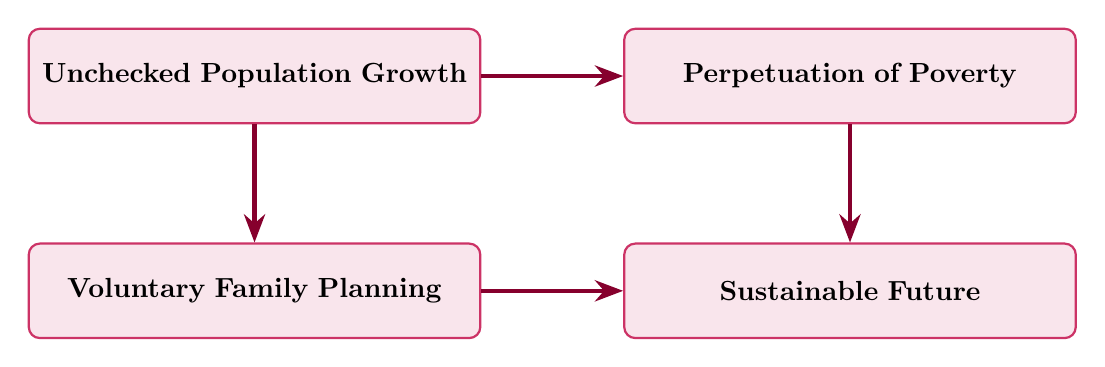
\begin{tikzpicture}[
    node distance=1.5cm,
    block/.style={rectangle, draw=purple!80, fill=purple!10, thick, rounded corners, text width=5.5cm, align=center, minimum height=1.2cm},
    arrow/.style={-Stealth, ultra thick, draw=purple!70!black}
]
    \node[block] (pop) {\textbf{Unchecked Population Growth}};
    \node[block, right=1.8cm of pop] (poverty) {\textbf{Perpetuation of Poverty}};
    \node[block, below=1.5cm of pop] (control) {\textbf{Voluntary Family Planning}};
    \node[block, below=1.5cm of poverty] (dev) {\textbf{Sustainable Future}};

    \draw[arrow] (pop) -- (poverty);
    \draw[arrow] (pop) -- (control);
    \draw[arrow] (poverty) -- (dev);
    \draw[arrow] (control) -- (dev);
\end{tikzpicture}
\caption{Page 40: The Population vs. Poverty Choice Cycle}
\end{figure}

\end{document}
\documentclass[12pt,a4paper]{article}
\usepackage[utf8]{utf8}
\usepackage[margin=1in]{geometry}
\usepackage{tcolorbox}
\usepackage{tikz}
\usetikzlibrary{shapes.geometric, arrows.meta, positioning}

\title{\textbf{The Ailing Planet: the Green Movement's Role}\\[0.3em] \Large Textbook Page 41 — Exercises}
\author{\textbf{Author:} Nani Palkhivala \quad|\quad \textbf{Textbook:} Hornbill (Class 11)}
\date{}

\begin{document}

\maketitle

\section*{Understanding the Text}

\begin{enumerate}
    \item Locate the lines in the text that support the title 'The Ailing Planet'.
    \item What does the notice 'The world's most dangerous animal' at a cage in the zoo at Lusaka, Zambia, signify?
    \item How are the earth's principal biological systems being depleted?
    \item Why does the author aver that the growth of world population is one of the strongest factors distorting the future of human society?
\end{enumerate}

\section*{Talking About the Text}

Discuss in groups of four:
\begin{enumerate}
    \item Laws are never respected nor enforced in India.
    \item "Are we to leave our successors a scorched planet of advancing deserts, impoverished landscapes and an ailing environment?"
    \item "We have not inherited this earth from our forefathers; we have borrowed it from our children".
    \item The problems of overpopulation that directly affect our everyday life.
\end{enumerate}

\vspace{1cm}

\begin{figure}[htbp]
\centering
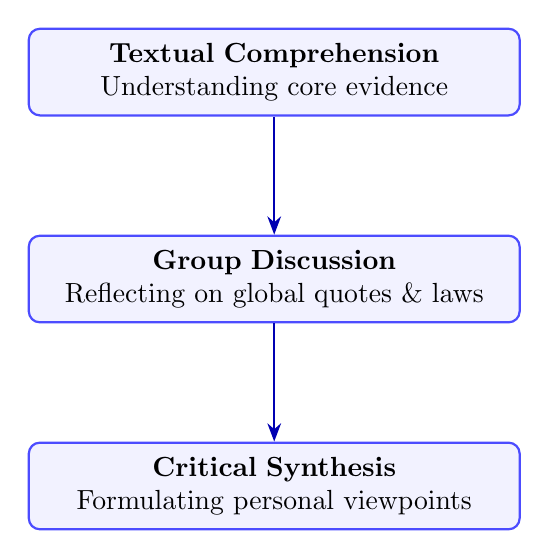
\begin{tikzpicture}[
    node distance=1.5cm,
    block/.style={rectangle, draw=blue!70, fill=blue!5, thick, rounded corners, text width=6cm, align=center, minimum height=1.1cm},
    arrow/.style={-Stealth, thick, draw=blue!70!black}
]
    \node[block] (t1) {\textbf{Textual Comprehension}\\ Understanding core evidence};
    \node[block, below=of t1] (t2) {\textbf{Group Discussion}\\ Reflecting on global quotes \& laws};
    \node[block, below=of t2] (t3) {\textbf{Critical Synthesis}\\ Formulating personal viewpoints};

    \draw[arrow] (t1) -- (t2);
    \draw[arrow] (t2) -- (t3);
\end{tikzpicture}
\caption{Page 41: Discussion \& Analysis Flowchart}
\end{figure}

\end{document}
\documentclass[12pt,a4paper]{article}
\usepackage[utf8]{utf8}
\usepackage[margin=1in]{geometry}
\usepackage{tcolorbox}
\usepackage{tikz}
\usetikzlibrary{shapes.geometric, arrows.meta, positioning}

\title{\textbf{The Ailing Planet: the Green Movement's Role}\\[0.3em] \Large Textbook Page 42 — Language \& Activities}
\author{\textbf{Author:} Nani Palkhivala \quad|\quad \textbf{Textbook:} Hornbill (Class 11)}
\date{}

\begin{document}

\maketitle

\section*{Thinking About Language}

The phrase 'inter alia' meaning 'among other things' is one of the many Latin expressions commonly used in English. Find out what these Latin phrases mean:
\begin{enumerate}
    \item \textit{prima facie}
    \item \textit{ad hoc}
    \item \textit{in camera}
    \item \textit{ad infinitum}
    \item \textit{mutatis mutandis}
    \item \textit{caveat}
    \item \textit{tabula rasa}
\end{enumerate}

\section*{Working With Words}

\subsection*{I. Connotations}
Locate the following phrases in the text and study their connotation:
\begin{itemize}
    \item gripped the imagination of
    \item dawned upon
    \item ushered in
\end{itemize}

\subsection*{II. Literal vs. Figurative Meanings}
The words 'grip', 'dawn', 'usher', 'coin', 'passport' have a literal as well as a figurative meaning. Write pairs of sentences using each word in the literal as well as the figurative sense.

\section*{Things to Do}

\begin{enumerate}
    \item Make posters to highlight the importance of the Green Movement.
    \item Maintain a record of the trees cut down and the parks demolished in your area, or any other act that violates the environment. Write to newspapers reporting on any such acts that disturb you.
\end{enumerate}

\vspace{1cm}

\begin{figure}[htbp]
\centering
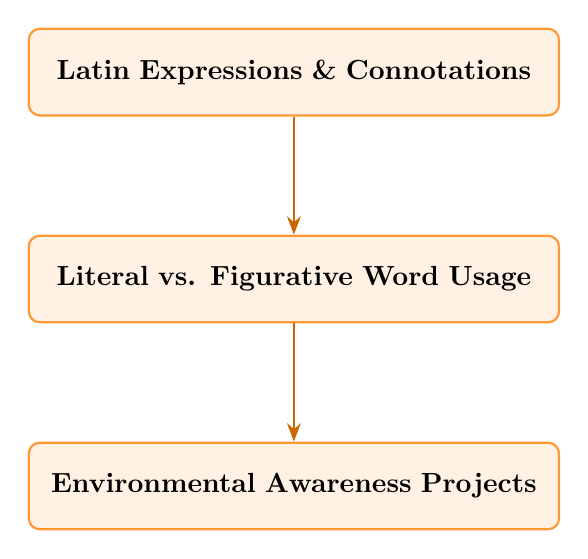
\begin{tikzpicture}[
    node distance=1.5cm,
    block/.style={rectangle, draw=orange!80, fill=orange!10, thick, rounded corners, text width=6.5cm, align=center, minimum height=1.1cm},
    arrow/.style={-Stealth, thick, draw=orange!80!black}
]
    \node[block] (lang) {\textbf{Latin Expressions \& Connotations}};
    \node[block, below=of lang] (fig) {\textbf{Literal vs. Figurative Word Usage}};
    \node[block, below=of fig] (act) {\textbf{Environmental Awareness Projects}};

    \draw[arrow] (lang) -- (fig);
    \draw[arrow] (fig) -- (act);
\end{tikzpicture}
\caption{Page 42: Linguistic & Action Framework}
\end{figure}

\end{document}

